\documentclass{beamer}
\usepackage[latin1]{inputenc}
\usetheme{CambridgeUS}
%\usetheme{Warsaw}
\usefonttheme[onlymath]{serif}
\title[MAB-based CMA-ES]{Multi-armed Bandit Based Covariance Matrix Adaptation
Evolution Strategy}
\author[Chuan-Che Yen]{Chuan-Che Yen \\Advisor: Dr. Tian-Li Yu}
\institute{TEILab}
\date{Nov 23, 2014}


%\setbeamercovered{transparent}
\usepackage{amsfonts}

%rendering images
\usepackage{graphicx}
\graphicspath{{./img/}}

%for algorithm
\usepackage[linesnumbered]{algorithm2e}

\AtBeginSection[]{
  \begin{frame}<beamer>
    \frametitle{Outline}
    \tableofcontents[
      currentsubsection,
      sectionstyle=show/shaded,
      subsectionstyle=show/show/hide,
    ]
  \end{frame}
}

\begin{document}

\begin{frame}
  \titlepage
\end{frame}
\begin{frame}
  \frametitle{Outline}
  \tableofcontents[
    currentsubsection,
    sectionstyle=show/show,
    subsectionstyle=show/hide,
  ]
\end{frame}





\section{Real-valued Function Optimization}

\begin{frame}{Real-valued Function Optimization}
  \begin{itemize}
    \item{Real-valued function}
      \begin{itemize}
        \item $f \colon \mathcal{S} \subset \mathbb{R}^n \to
          \mathbb{R},x \mapsto f(x)$
        \item $\mathcal{S} \colon $ search space
        \item Elements of $\mathcal{S} \colon $ candidates or solutions
      \end{itemize}
    \item{Optimization}
      \begin{itemize}
        \item $\mathop{\arg\min}\limits_{x} f(x)$, where $x$ are within given bounds.
        \item Maximizing $f$ is equivalent to minimizing $-f$.
      \end{itemize}
    \item Example
      \begin{itemize}
        \item $\mathop{\arg\min}\limits_x 2x^3-3x^2-36x-14$.
        \item Design of aircraft wings.
      \end{itemize}
  \end{itemize}
\end{frame}

\begin{frame}{Black-box Optimization}

  \begin{figure}[h]
    \includegraphics[scale=0.5]{BlackBox.eps}
    \caption{Black-box function}  
  \end{figure}
  \begin{itemize}
    \item The only information is the interaction between input and
    output.  
  \item The key point is investigating the trade-off between
    \alert{exploration}
    and \alert{exploitation}.
    \begin{itemize}
      \item Exploration is the capability of \alert{having an overview for the search
        space}.
  \item Exploitation is the capability of \alert{generating high resolution
    candidates}. 
    \end{itemize}
  \end{itemize}

\end{frame}

\begin{frame}{Difficulties}
  \begin{columns}
    \begin{column}{0.6\textwidth}
      \begin{itemize}[<+->]
        \item Non-convex
          \begin{itemize}
            \item Local optima are less important for global optimum.
          \end{itemize}
        \item Ruggedness
          \begin{itemize}  
            \item Perturbated by noise. 
            \item Non-smooth.
          \end{itemize}
        \item Dimensionality
          \begin{itemize}
            \item Search space grows exponentially
          \end{itemize}
        \item Non-separable
          \begin{itemize}
            \item Dependencies between decision variables
          \end{itemize}
        \item Ill-conditioned
          \begin{itemize}
            \item Unable to extract gradient information
          \end{itemize}
      \end{itemize}
    \end{column}
    \begin{column}{0.4\textwidth}
      \onslide<2->{
        \begin{figure}[l]
          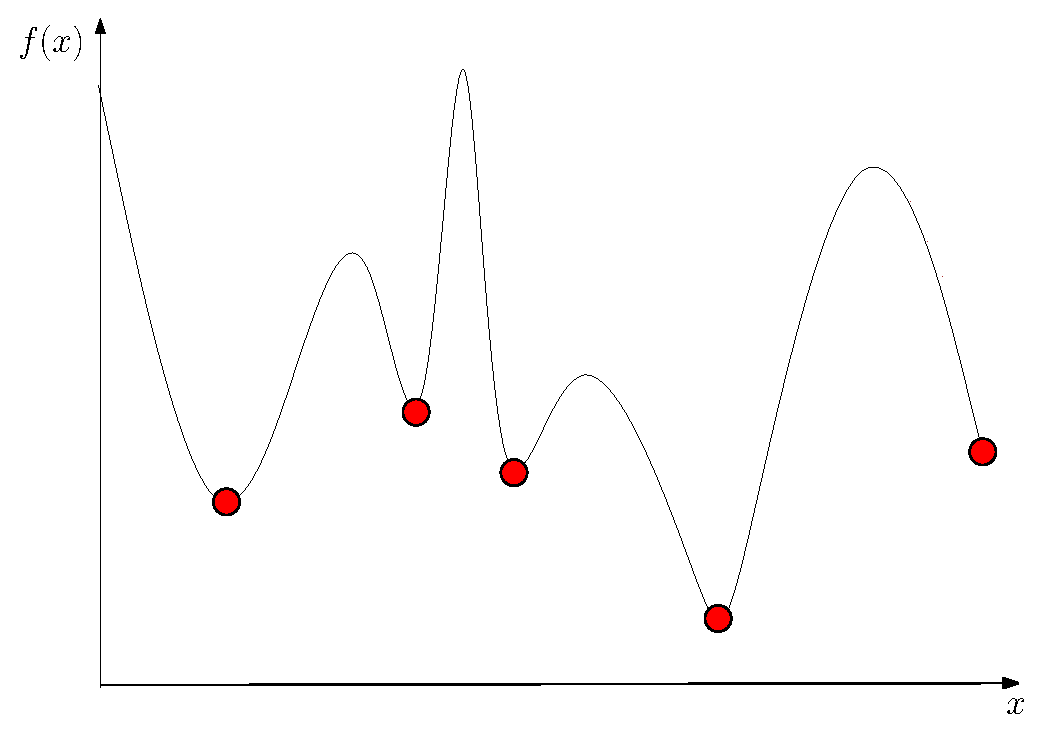
\includegraphics[width = 0.6\columnwidth]{Non-Convex.eps}
          \caption{Non-convex function}
        \end{figure}
      }
      \onslide<4->{
        \begin{figure}[H]
          \includegraphics[width = 0.6\columnwidth]{Rugged.eps}
          \caption{$sin(x)$ with noise}
        \end{figure}
      }
    \end{column}
  \end{columns}
\end{frame}

\section{Related Approaches}
\begin{frame}{Related Approaches}
  \begin{itemize}
    \item Optimization
      \begin{itemize}
        \item Deterministic
        \item Stochastic
      \end{itemize}
      \vspace*{14pt}
    \item Properties
      \begin{itemize}
        \item Stability
        \item Robustness
      \end{itemize}
      \vspace*{14pt}
    \item Utilizing global information
      \begin{itemize}
        \item Estimation of Distribution Algorithm (EDA)
        \item Model building
      \end{itemize}
  \end{itemize}
\end{frame}

\subsection{Real-coded Extended Compact Genetic Algorithm}


\begin{frame}{Discretization} 
  \begin{itemize} 
    \item Continuous domain $\rightarrow$ Discrete domain 
    \item Finding good solutions $\rightarrow$ Finding promising
      regions
    \item 2 traditional discretization methods
      \begin{itemize}
        \item Fixed-Height Histogram (FHH)
        \item Fixed-Width Histogram (FWH)
      \end{itemize}
      \vspace*{2pt}
  \end{itemize}
  \begin{minipage}{.45\textwidth}
    \begin{figure}
      \centering
      \includegraphics[width =0.5\linewidth]{FHH.eps}
      \caption{Illustration of FHH}
    \end{figure}
  \end{minipage}
  \begin{minipage}{.45\textwidth}
    \begin{figure}
      \centering
      \includegraphics[width =0.5\linewidth]{FWH.eps}
      \caption{Illustration of FWH}
    \end{figure}
  \end{minipage}

\end{frame}

\begin{frame}{Split on Demand}
  \begin{itemize}
    \item Solutions in each bin should not exceed $\gamma N$.
      \begin{itemize}
        \item $N$ is the population size.
        \item $\gamma$ defines the rate of one region.
      \end{itemize}
    \item $\gamma$ decays with a factor $\epsilon$.
  \end{itemize}
  \hspace{-9cm}
  \vspace*{-0.5cm}
  \begin{figure}[h]
    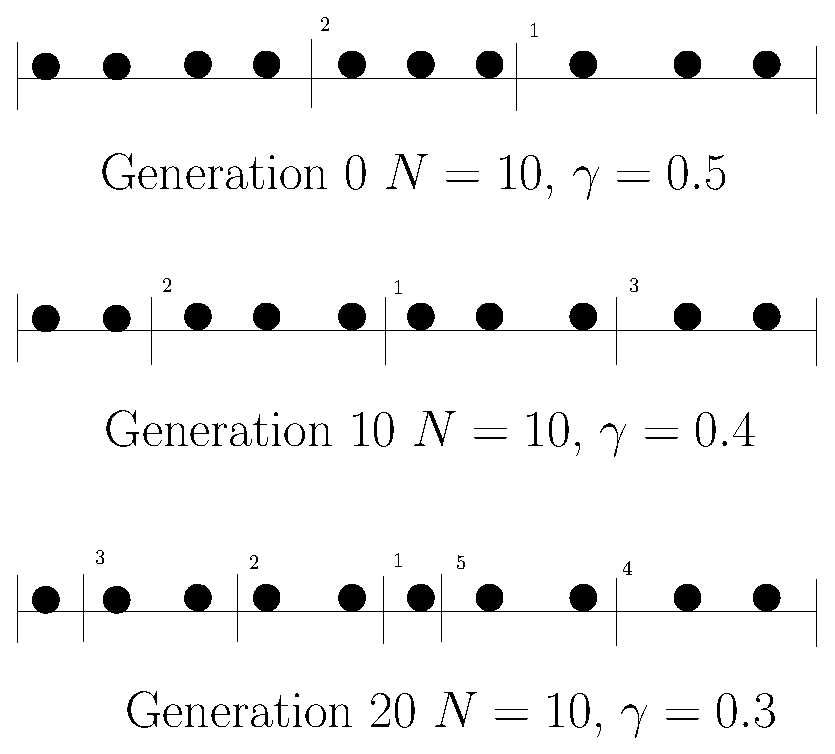
\includegraphics[scale = 0.2]{SoD.eps}
    \caption{Illustration of SoD}
  \end{figure}
\end{frame}

\begin{frame}{EDA}
  \begin{columns}
    \begin{column}{.65\textwidth}
      \begin{itemize}
        \item Sometimes known as Probabilistic Model Building GA (PMBGA).
          \begin{itemize}
            \item Building model explicitly.
            \item Linkage between decision variables are provided.
          \end{itemize}
          \vspace*{14pt}
        \item  Extended Compact Genetic Algorithm (ECGA).
          \begin{itemize}
            \item Model is built according to population distribution.
            \item Applying greedy search to refine model iteratively.
          \end{itemize}
         % \begin{figure}
         %   \centering
         %   \only<4>{\includegraphics[height = 0.5\textheight]{EDA.eps}}
         % \end{figure}
      \end{itemize}
    \end{column}
    \begin{column}{.35\textwidth}
      \begin{figure}[htp]
        \centering
        \includegraphics[width = 0.8\textwidth]{EDA.eps}
        \caption{EDA}
      \end{figure}
    \end{column}
  \end{columns}
\end{frame}

\begin{frame}{Real-coded ECGA with SoD}
  \vspace*{14pt}
  \begin{figure}
    \flushleft
    
    \includegraphics[width=.6\textwidth]{rECGA.eps}
    \caption{rECGA}
  \end{figure}
  %\pause
  %\begin{enumerate}
  %  \item Preparing discretization\pause
  %    \vspace*{14pt}
  %  \item Integrating discretized results into ECGA.\pause
  %    \vspace*{14pt}
  %  \item ECGA builds model accordingly, output the promising
  %    regions.\pause
  %    \vspace*{14pt}
  %  \item Sampling accordingly.\pause
  %    \vspace*{14pt}
  %  \item For every $L$ generations, a local optimizer is adopted to
  %    obtain high resolution solutions\pause
  %    \vspace*{14pt}
  %  \item If model does not converge, goto 1.
  %\end{enumerate}
\end{frame}

\subsection{Covariance Matrix Adaptation Evolution Strategy}


\begin{frame}{Evolution Strategy (ES)}
  \begin{itemize}
    \item A search template for black-box optimization.
      \begin{itemize}
        \item Encoded in continuous domain.
      \end{itemize}
      \vspace*{14pt}
    \item New search points are generated based on current population.
      \vspace*{14pt}
    \item $(\mu,\lambda)$-ES and $(\mu+\lambda)$-ES.
      \vspace*{14pt}
    \item $x_i^{t+1} = m^t + \sigma N_i(0,C)$.
      \begin{itemize}
        \item $x_i^{t+1}$: $i$-th generated solution at generation $t+1$.
        \item $m^t$: weighted mean of population at generation $t$.
        \item $\sigma$: step size.
        \item $C$: Estimated distribution.
      \end{itemize}
  \end{itemize}
\end{frame}

\begin{frame}{Covariance Matrix Adaptation Evolution Strategy (CMA-ES)}
  \begin{itemize}
    \item A famous branch of ES.
      \vspace*{14pt}
    \item Importance of $\sigma$ and $C$.
      \begin{itemize}
        \item Larger step size reinforces exploration while smaller
          reinforces exploitation.
          \begin{itemize}
            \item Choosing an fixed, appropriate number?
          \end{itemize}
        \item Covariance matrix determines the shape of estimated
          distribution.
          \begin{itemize}
            \item Determining the length of each axis.
            \item Representing the dependency among decision variables.
          \end{itemize}
      \end{itemize}
      \vspace*{14pt}
    \item CMA-ES features in the adoption of historical information.
      \begin{itemize}
        \item $\sigma$ and $C$ are adjusted accordingly.
      \end{itemize}
  \end{itemize}
\end{frame}

\begin{frame}{Illustration of CMA-ES}
  \begin{figure}
    \includegraphics[scale = 0.4]{CMAES.eps}
  \end{figure}
%  \begin{columns}
%    \begin{column}{.33\textwidth}
%      \begin{figure}
%        \centering
%        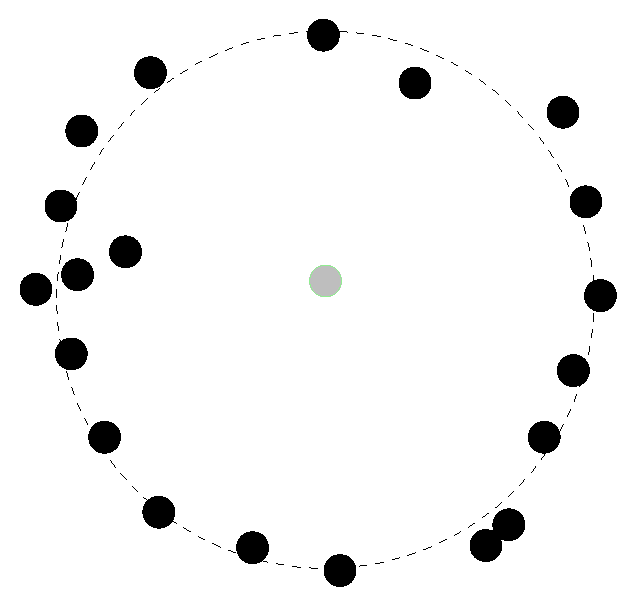
\includegraphics[width=.9\textwidth]{ES_0.eps}
%        \caption{$t$ = 0}
%      \end{figure}
%    \end{column}
%    \begin{column}{.33\textwidth}
%      \begin{figure}
%        \centering
%        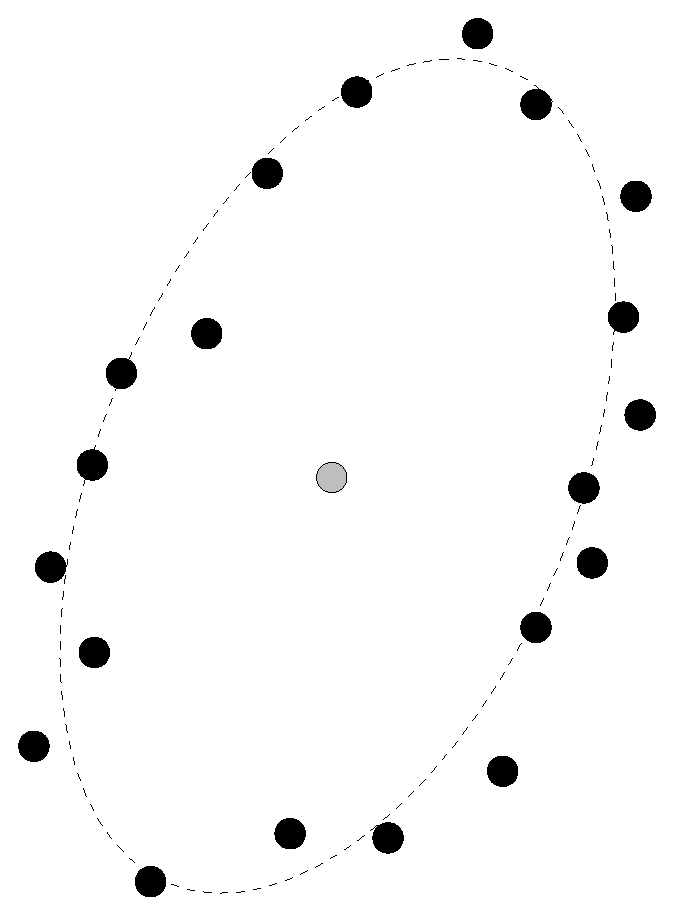
\includegraphics[width=.9\textwidth]{ES_10.eps}
%        \caption{$t$ = 10}
%      \end{figure}
%    \end{column}
%    \begin{column}{.33\textwidth}
%      \begin{figure}
%        \centering
%        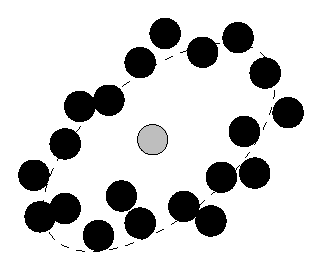
\includegraphics[width = .9\textwidth]{ES_20.eps}
%        \caption{$t$ = 20}
%      \end{figure}
%    \end{column}
%  \end{columns}
\end{frame}


%\section{Motivation}

\begin{frame}{rECGA}
  \begin{itemize}
    \item Discretization 
      \begin{itemize}
        \item Continuous domain $\rightarrow$ Discrete domain $\rightarrow$
          Continuous domain
        \item Is there any distortion?
      \end{itemize}
  \end{itemize}
  \vspace*{24pt}
  \begin{figure}[htpb]
    \includegraphics[width = 0.4\textwidth]{Discretization.eps}
  \end{figure}
\end{frame}

\begin{frame}{rECGA}
  \begin{itemize}
    \item Unreasonable sampling
      \begin{itemize}
        \item The cliff between each bin is sometimes steep.
      \end{itemize}
  \end{itemize}
  \begin{figure}[hpb]
    \centering
    \vfill\includegraphics[width = 0.4\textwidth]{Sampling.eps}
  \end{figure}
\end{frame}

\begin{frame}{rECGA}
  \begin{itemize}
    \item rECGA tackles the difficulty of
      \alert{non-separable} and \alert{Ill-conditioned}.
      \vspace*{14pt}
    \item rECGA limits the searching region in early stage to deal with
      \alert{dimensionality}.
      \vspace*{14pt}
    \item rECGA struggles in exploration and encounters the previous
      introduced hazard.
      \vspace*{14pt}
    \item Why not make real-valued problem solved by methods encoded in
      continuous domain?

  \end{itemize}
\end{frame}
\begin{frame}{CMA-ES}
  \begin{itemize}
    \item An outstanding local optimizer
    \item Tackles \alert{non-separable} by maintaining a
      covariance matrix
    \item Usually encounters premature convergence
  \end{itemize}
  \begin{figure}[htpb]
    \centering
    \vfill\includegraphics[scale = 0.3]{LocalOptima.eps}
  \end{figure}
\end{frame}
\begin{frame}{Hypothesis}
  \begin{itemize}
    \item Both CMA-ES and rECGA suffer from \alert{ruggedness} for
      insufficient exploration.
      \vspace*{8pt}
    \item What if there is implicit information between local optima?
    \item We are interested in rugged problems with implicit tendency
  \end{itemize}
  \vspace*{10pt}
  \begin{figure}[hp]
    \centering
    \includegraphics[scale=0.3]{Problem.eps}
  \end{figure}
\end{frame}

\begin{frame}{Hypothesis}
  \begin{itemize}
    \item Assume problems are with such structure
      \vspace*{10pt}
    \item We are aiming to fetch more promising region by evolving the
      tendency
  \end{itemize}
  \vspace*{10pt}
  \begin{figure}[hp]
    \centering
    \includegraphics[scale=0.3]{tendency.eps}
  \end{figure}
\end{frame}
\begin{frame}{Hypothesis}
  \begin{itemize}
    \item A reasonable discretization 
      \vspace*{10pt}
    \item Clustering based on space locality  
  \vspace*{10pt}
\item Performing a 2nd layer CMA-ES for evolving the tendency
  \end{itemize}
  \vspace*{10pt}
  \begin{figure}[htpb]
    \centering
    \includegraphics[scale=0.35]{hypothesis_discretization.eps}
  \end{figure}
\end{frame}

\begin{frame}{Expected benefit}
  \begin{itemize}
    \item A soft, adaptive discretization
      \begin{itemize}
        \item Iteratively exploring better regions.
        \item Generated regions are also source for better regions.
      \end{itemize}
      \vspace*{14pt}
    \item Each region can be highly exploited. 
      \begin{itemize}
        \item 1st layer CMA-ES quickly outputs local optimum.
      \end{itemize}
  \end{itemize}
\end{frame}




%\begin{frame}{Hypothesis}
%
%  \begin{itemize}
%    \item Increasing diversity by maintaining multiple groups.
%      \begin{itemize}
%        \item kind of discretization.
%        \item How to define the number of groups?
%        \item What is the criteria for individuals to form a group?
%      \end{itemize}
%      \vspace*{14pt}
%    \item There is implicit information hidden between groups.
%      \begin{itemize}
%        \item How to extract the information?
%        \item How to benefit from the information and obtain
%          better solutions?
%          \begin{itemize}
%            \item Inspired by discretization, we aim to find a more
%              promising region.
%          \end{itemize}
%      \end{itemize}
%      \vspace*{14pt}
%    \item 2-layer CMA-ES is introduced
%      \begin{itemize}
%        \item Inner layer for exploitation
%        \item Outer layer for exploration
%      \end{itemize}
%  \end{itemize}

%\end{frame}

%\section{Methodology}

\begin{frame}{Flow of Proposed Template}
  \begin{columns}
    \begin{column}{0.9\textwidth}
      \begin{figure}[b]
        \vspace*{1cm}        
        \includegraphics[width = 0.6\textwidth]{Flow.eps}\hspace*{2cm}
        \caption{Flow}
      \end{figure}
    \end{column}
  \end{columns}
\end{frame}

\begin{frame}
  \frametitle{Pseudo-code of Template}

  \scalebox{0.8}{%
    \begin{algorithm}[H]
      \Begin{
        Initializing population\;
        Clustering\;
        \While{not terminate}{
          \While{any group has not been evolved for certain generation}{
            Evolving each group\;
          }
          Selecting candidates for each group\;
          Evolving the selected solutions\;
        } 
      }
      \TitleOfAlgo{Overview for the system}
    \end{algorithm}
  }
\end{frame}   

\begin{frame}{Undetermined Components}
  \begin{itemize}
    \item The method for making division
      \vspace*{14pt}
    \item The criterion of selecting representative solutions for
      each group
      \vspace*{14pt}
    \item The method for evolving the selected candidates
  \end{itemize}
\end{frame}

\begin{frame}{Making Division}
  \begin{itemize}
    \item The initial population is expected to categorized according to position.
      \begin{itemize}
        \item Roughly expresses the diversity
        \item A population in a specific region is expected driven
          toward the identical local optimum.
        \item In other words, a group can be roughly viewed as points
          near by one specific valley. 
      \end{itemize}
      \vspace*{14pt}
    \item Space locality plays an important role.
      \begin{itemize}
        \item Applying clustering
      \end{itemize}
  \end{itemize}
\end{frame}

\begin{frame}{\emph{k-means}}
  \begin{itemize}
    \item \emph{k-means} clustering is a basic method for vector quantization.
      \begin{itemize}
        \item Partitioning $n$ solutions into $k$ mutual independent
          clusters.
        \item Serving as a prototype
      \end{itemize}
      \vspace*{14pt}
    \item Number of clusters
      \begin{itemize}
        \item As known as number of groups.
        \item Without $k$, finding optimal is said to be NP-hard.  
        \item To define a proper $k$ is difficult.
      \end{itemize}
      \vspace*{14pt}
    \item  Heuristic algorithms for approximation.
      \begin{itemize}
        \item Forgy method for initialization
        \item iteratively refinements until convergence
      \end{itemize}

  \end{itemize}
\end{frame}

\begin{frame}{Algorithm of Approximation to k-means}

  \scalebox{0.8}{%  
    \begin{algorithm}[H]
      \label{algo:kmeans}
      \KwIn{$k$, $d$, $\{o_1, o_2,\ldots, o_n\}$ as observations} 
      \KwOut{$\mathcal{S}$} 
      Initial: $m_1, m_2,\ldots, m_k$ are
      random selected from observations as initial centers 
      \tcp*{Forgy method}
      \While{At least one of the observations moves to other group} 
      {\For{j = 1 to k} 
      {$S_j = \emptyset$  \;} 
      \For{i = 1 to n} {assign $o_i$ to $S_j$ if $o_i$ is
      closest to $m_j$ among the $k$ centers\;} 
      \For{j = 1 to k} {$m_j$ is updated by the arithmetic mean of all vectors $\in S_j$\;}
    }
    \TitleOfAlgo{Clustering heuristic function}
  \end{algorithm}
}

\end{frame}

\begin{frame}{Illustration for The Algorithm}
  \begin{columns}

    \begin{column}{0.23\textwidth}
      \begin{figure}[h]
        \centering
        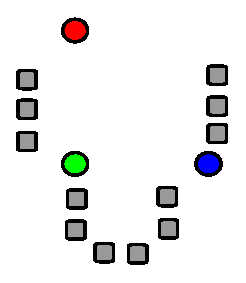
\includegraphics[scale = 0.5]{K_Means_Example_Step_1.eps}
      \end{figure}
    \end{column}

    \begin{column}{0.23\textwidth}
      \begin{figure}[h]
        \centering
        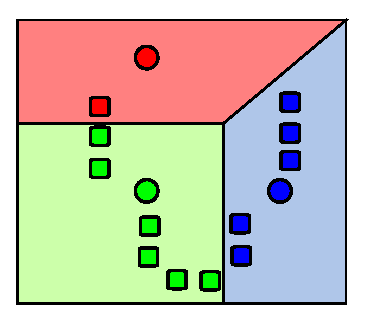
\includegraphics[scale = 0.5]{K_Means_Example_Step_2.eps}
      \end{figure}
    \end{column}

    \begin{column}{0.23\textwidth}
      \begin{figure}[h]
        \centering
        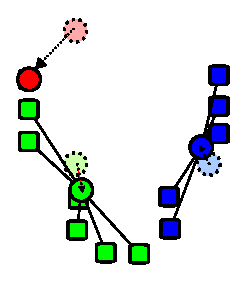
\includegraphics[scale=0.5]{K_Means_Example_Step_3.eps}
      \end{figure}
    \end{column}

    \begin{column}{0.23\textwidth}
      \begin{figure}[h]
        \centering
        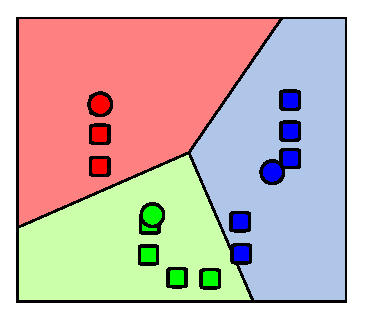
\includegraphics[scale = 0.5]{K_Means_Example_Step_4.eps}
      \end{figure}
    \end{column}
  \end{columns}
\end{frame}

\begin{frame}{Remaining Criteria}
  \begin{itemize}
    \item How to select representativeness from each group?
      \begin{itemize}
        \item Using the optimal solution found so far as the representativeness in
          each group
      \end{itemize}
      \vspace*{14pt}
    \item How to evolve selected candidates?
      \begin{itemize}
        \item Evolving them with CMA-ES
        \item The so-called `outer CMA-ES'
        \item Aims to observe if better regions can be reached
      \end{itemize}
      \vspace*{14pt}
    \item The number of solutions in a group is fixed after clustering.
      \begin{itemize}
        \item Once a better solution is generated, the worst one should
          be replaced.
      \end{itemize}
  \end{itemize}
\end{frame}

\begin{frame}{An Implementation of the Template}
  \scalebox{0.8}
  {
    \begin{algorithm}[H]{
        \KwIn{$n$,$t$}
        \KwOut{best solution ever evolved}
        Uniformly sampled population of size $n$\;
        $k = \sqrt{\frac{n}{2}}$\;
        Integrating \emph{k-means} with \emph{Frogy-method} to cluster the
        $n$ individuals into $k$ groups\;

        $C\leftarrow$ array with size $k$\;
        \For{i = 1 to k}
        {
          Optimizing group$_i$ by adopting CMA-ES for $t$ generations\;
          $C_i\leftarrow$ best solution\;
          Applying CMA-ES to evolve the population consisting of local
          optima of groups, as known as $C$, until terminated.\;
        }
      }
      \TitleOfAlgo{2-layer CMA-ES}
    \end{algorithm} 
  }
\end{frame}

\begin{frame}
  \begin{itemize}
    \item 2-layer CMA-ES addresses the diversity for the search.
      \vspace*{14pt}
    \item Next we lay emphasis on finding more promising regions.
  \end{itemize}

\end{frame}

\begin{frame}{Exploring}
  \begin{itemize}
    \item Based on current groups, we aim to figure out better
      solutions.
      \begin{itemize}
        \item According to our hypothesis, the implicit information is
          hidden between groups.
        \item What is a good way to evolve groups?
      \end{itemize}
      \vspace*{14pt}
    \item We consider the priority
      \begin{itemize}
        \item Put less concentration on groups which performs badly
        \item Lay emphasis on possible regions
        \item Without any prior knowledge, a selection strategy is
          demanded.
      \end{itemize}
      \vspace*{14pt}
    \item The ability to generate new groups adaptively 
      \begin{itemize}
        \item We assume a fixed number of groups.
        \item A replacement strategy is demanded accordingly.
      \end{itemize}
  \end{itemize}
\end{frame}

\begin{frame}{The Selection Strategy}

  \begin{itemize}
    \item The selection strategy is with the feature that
      \begin{itemize}
        \item Given a set of groups, the performance of each group is
          evaluated through trials
        \item Lays emphasis on better performance groups
        \item groups with worse performance would not be ignored
          permanently
      \end{itemize}
      \vspace*{14pt}
    \item This is just identical to the Multi-armed Bandit (MAB)
      problem.
  \end{itemize}
\end{frame}

\begin{frame}{Multi-armed Bandit Problem}
  \begin{itemize}
    \item Investigate the trade-off between exploration and exploitation
      \vspace*{14pt}
    \item Assume there are $k$ independent slot machines
      \vspace*{14pt}
    \item Each machine generates reward according to its own unknown probability
      distribution.
      \vspace*{14pt}
    \item We can only observe the playing sequence and the correlated
      reward.
      \vspace*{14pt}
    \item The goal is to maximize reward in limited play times.
  \end{itemize}
\end{frame}

\begin{frame}{Upper Confidence Bound }
  \begin{itemize}
    \item A family of solutions to MAB problems
      \vspace*{14pt}
    \item UCB1 -- the first Upper Confidence Bound (UCB) algorithm
      \vspace*{14pt}
    \item Play machine $j$ which maximizes
      \[\bar{x_j} + \sqrt{\frac{2\ln n}{n_j}}\]
      \begin{itemize}
        \item $\bar{x_j}$: the average reward of machine $j$.
        \item $n_j$: the number of times machine $j$ has been played.
        \item $n$: the played times of overall system.
      \end{itemize} 
  \end{itemize}
\end{frame}

\begin{frame}{UCB1-tuned}
  \begin{itemize}
    \item UCB1 takes no variance into consider.
      \begin{itemize}
        \item UCB1-tuned is the version which adds variance as a factor.
        \item UCB1-tuned is not proven working well but outperforms UCB1 in
          practice.
        \item In UCB1-tuned, the machine $j$ to be played is with the
          highest \[\bar{x_j} + \sqrt{\frac{\ln{n}}{n_j}
          \min(\frac{1}{4},V_j(n_j))}\], where $V_j(t) =\sigma_j^2 +
          \sqrt{\frac{2\ln n}{n_j}}$.
      \end{itemize}
      \vspace*{14pt}
    \item UCB1-tuned is adopted in our work.
  \end{itemize}

\end{frame}

\begin{frame}{The Replacement Strategy}
  \begin{itemize}
    \item By generating a new point and sampling around the new point,
      we claim to form a better group, and the worst one should be
      replaced.
      \vspace*{14pt}
    \item There are 2 judgement to distinguish if there is any group to
      delete.
      \begin{enumerate}
        \item If a group does not sample a better solution anyway.
        \item If no group converges, check among groups if there is
          group has not been played for $t$ rounds where $t$ is a
          number larger than the number of the solutions the group
          contains.
      \end{enumerate}
  \end{itemize}
\end{frame}

\begin{frame}{Flow of MAB-based CMA-ES}
  \begin{figure}[h]
    \vspace{15mm}\includegraphics[scale=0.4]{FlowMAB.eps}\hspace{25mm}
  \end{figure}
\end{frame}

\begin{frame}{Procedure of MAB-based CMA-ES}
  \scalebox{0.7}{
    \begin{algorithm}[H] 
      \TitleOfAlgo{MAB-based CMA-ES} 
      \KwIn{$n$,$t$ as a proper generation for each pulling action}
      \KwOut{best solution ever evolved} 
      Uniformly sampled population of size $n$\; 
      $k = \sqrt{\frac{n}{2}}$\; 
      Integrating \emph{k-means} with \emph{Frogy-method} to cluster the $n$ individuals into
      $k$  groups as known as bandits\; 
      $C\leftarrow$ array with size $k$\;
      \For{i = 1 to k}            
      { pull($i$)\; $C_i\leftarrow$ best
      solution\; } 
      \While{not terminated} 
      { \For{i = 1 to k} {
        calculateUCB($i$) \tcp*[r]{calculate modified UCB1-tuned as
        illustrated above} record the index with max value in $M$\;

      } 
      pull($M$)\;      
      $C_M \leftarrow$ best solution in
    group$_M$\; update()\; }
  \end{algorithm}  }
\end{frame}

\begin{frame}
  \scalebox{0.65}{
    \begin{algorithm}[H]
      Initial $P\leftarrow $ a permutation array from $1$ to $k$\; 
      ToBeDeleted = $0$\;
      \For{i = 1 to k} 
      {
        \If{deleting criterion 1 is met in group$_{P_i}$} 
        {
          ToBeDeleted = $P_i$\; 
        }  

      }
      \If{ToBeDeleted = 0} 
      {
        \For{i = 1 to k} 
        {
          \If{deleting criterion 2 is met in group$_{P_i}$}
          {
            ToBeDeleted = $P_i$\;
          } 
        } 
      } 
      \If{ToBeDeleted = 0} 
      { 
        return\; 
      } 
      \Else
      { 
        $s\leftarrow$ ToBeDeleted\; 
        generate a new solution as a new group  denoted as $group^\star$ according to $C_1, C_2,\ldots, C_{s_{i-1}}, C_{s_{i+1}},\ldots, C_k$ \; 
        \For{i = 1 to $\|group_{s}\|-1$} 
        { pull($group^\star$) without replacing worst\; }
        replace $group_{s}$ with $group^\star$\; return\; 
      } 
      \TitleOfAlgo{update}
    \end{algorithm} 
  }
\end{frame}

%\section{Experiments and Results}

\begin{frame}{Testbed}
  \begin{figure}
    \centering
  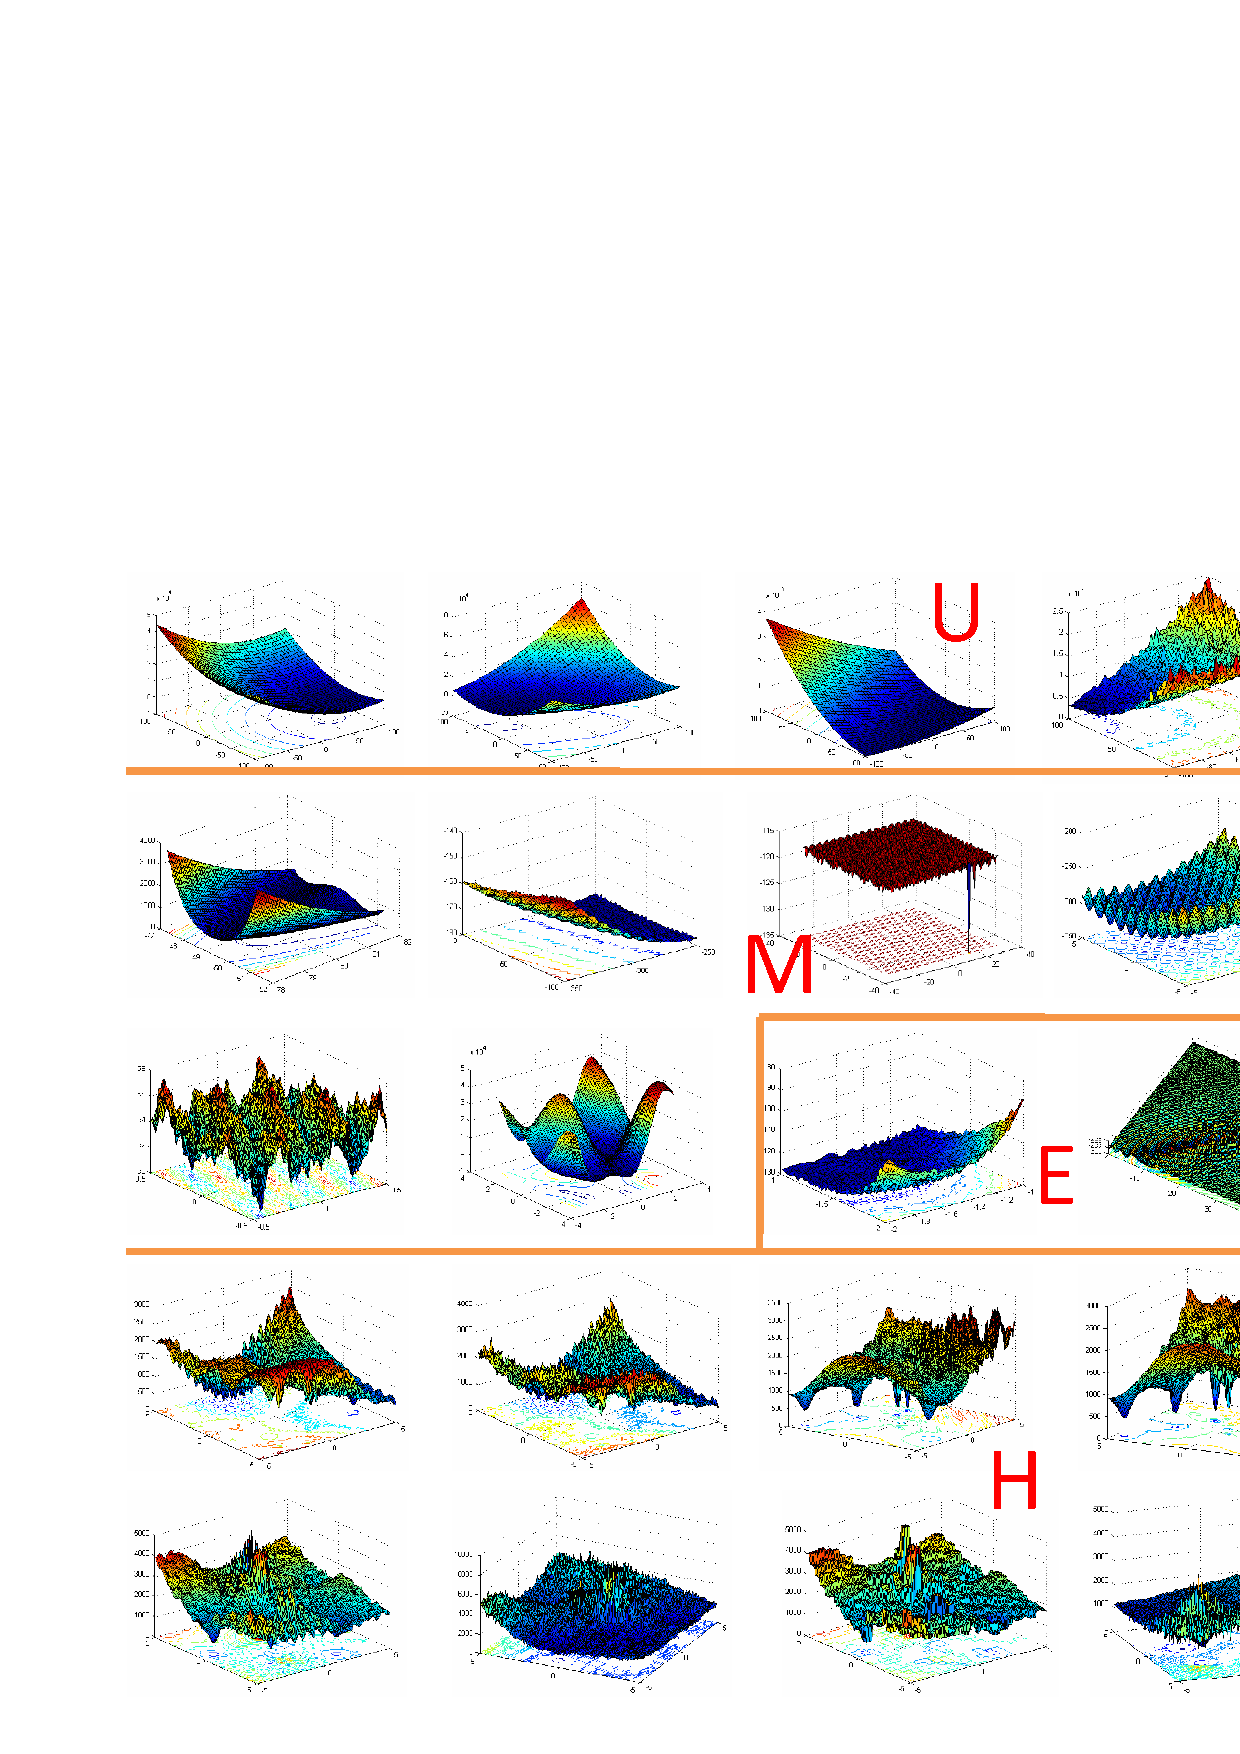
\includegraphics[bb= 43 16 783 584, clip, width =.8\textwidth]{benchmark}
\end{figure}
\end{frame}

\begin{frame}{Testbed}
  \begin{itemize}
    \item A set of benchmark proposed in CEC 2005 (Suganthan et al. 2005) 
      \vspace*{14pt}
    \item 25 problems are categorized into 4 kinds of problem that
      \begin{itemize}
        \item \alert{U}nimodal functions (1--5)
        \item \alert{M}ulti-modal functions (6--12)
        \item \alert{E}xpanded functions (13--14)
        \item \alert{H}ybrid composition functions (15--25)
      \end{itemize}
      \vspace*{14pt}
    \item Benchmark criteria
      \begin{itemize}
        \item The best accuracy after $10^5$ function evaluations
      \end{itemize}
  \end{itemize}
\end{frame}


\begin{frame}{Experiments Design}
  \begin{itemize}
    \item Comparison for robustness is performed
      \vspace*{14pt}
    \item 2 comparisons
      \begin{enumerate}
        \item Comparing to original CMA-ES 
        \item Comparing to rECGA + SoD
      \end{enumerate}
      \vspace*{14pt}
    \item The judging criteria
      \begin{itemize}
        \item Each problem runs 25 times.
        \item The best, median, worst solutions of each run are collected.
      \end{itemize}
  \end{itemize}
\end{frame}

\begin{frame}{Comparison to Original CMA-ES}
  \begin{itemize}
    \item For all instance of CMA-ES, $\lambda = 20$ and $\sigma$ is
      initial to $1$.
    \item For each pull option, the 1st layer CMA-ES executes for $30$
      iterations.
    \item The population size is set to be $450$ and $k = 15$ for
      MAB based CMA-ES.
  \end{itemize}
  \begin{columns}
    \footnotesize
    \begin{column}{0.5\textwidth}
\begin{table}[h]
\begin{tabular}{|c|c|c|}
\hline
      & \begin{tabular}[c]{@{}c@{}}Original\\ CMA-ES\end{tabular} & \begin{tabular}[c]{@{}c@{}}MAB-basd\\ CMA-ES\end{tabular} \\ \hline
U     & --                                                       & --              \\ \hline
M     & --                                                       & 1               \\ \hline
E     & --                                                       & 2               \\ \hline
H     & --                                                       & 6               \\ \hline
Total & --                                                       & 9               \\ \hline
\end{tabular}
\caption{Comparison of best run}
\end{table}
      
    \end{column}
\begin{column}{0.5\textwidth}
\begin{table}[h]
\begin{tabular}{|c|c|c|}
\hline
      & \begin{tabular}[c]{@{}c@{}}Original\\ CMA-ES\end{tabular} & \begin{tabular}[c]{@{}c@{}}MAB-basd\\ CMA-ES\end{tabular} \\ \hline
U     & --
& --                                                         \\ \hline
M     & --
& 3                                                         \\ \hline
E     & --                                                       & 2                                                         \\ \hline
H     & 1
& 9                                                         \\ \hline
Total & 1                                                        &
14                                                        \\ \hline
\end{tabular}
\caption{Comparison of median run}
\end{table}
\end{column}
  \end{columns}

\end{frame}
\begin{frame}{Comparison to rECGA + SoD}
  \begin{itemize}
    \item Same settings as SoD paper
  \end{itemize}
\begin{columns}
\begin{column}{0.5\textwidth}
\begin{table}[h]
\begin{tabular}{|c|c|c|}
\hline
      & \begin{tabular}[c]{@{}c@{}}rECGA+\\ SoD\end{tabular} & \begin{tabular}[c]{@{}c@{}}MAB-basd\\ CMA-ES\end{tabular} \\ \hline
U     & --
& 5                                                    \\ \hline
M     & 1                                                         &
5                                                    \\ \hline
E     & 2                                                         &
--                                                    \\ \hline
H     & 4                                                         & 4                                                    \\ \hline
Total & 7                                                        &
14                                                   \\ \hline
\end{tabular}
\caption{Comparison of best run}
\end{table}
\end{column}
\begin{column}{0.5\textwidth}
 \begin{table}[h]
\begin{tabular}{|c|c|c|}
\hline
      & \begin{tabular}[c]{@{}c@{}}rECGA+\\ SoD\end{tabular} & \begin{tabular}[c]{@{}c@{}}MAB-basd\\ CMA-ES\end{tabular} \\ \hline
U     & --
& 5                                                    \\ \hline
M     & 1
& 5                                                    \\ \hline
E     & 2
& --                                                    \\ \hline
H     & 2
& 8                                                    \\ \hline
Total & 5
& 18                                                    \\ \hline
\end{tabular}
\caption{Comparison of median run}
\end{table} 
\end{column}

\end{columns}

\end{frame}
\begin{frame}{Discussion}
 
  \begin{itemize}
    \item Strength
      \begin{itemize}
        \item Higher median values in 18 problems comparing to rECGA+SoD.
        \item Higher median values in all multimodel problems except
          problem 22 compaing to CMA-ES
      \end{itemize}
      \vspace*{14pt}
    \item Weakness
      \begin{itemize}
        \item Reach no global optimum in problems addressed by a dence
          distribution of local optima.
        \item Too complicated for simple problem.
      \end{itemize}
      \vspace*{14pt}
    \item Improvement
      \begin{itemize}
        \item Ruggedness
        \item Non-convex
      \end{itemize}

  \end{itemize}

\end{frame}
%\begin{frame}{Comparison}
%  \begin{itemize}
%    \item For original CMA-ES, the $\lambda$ is set to 20 and $\sigma$
%      is initialized to 1.
%    \item For 2-layer CMA-ES, the $\lambda$ and $\sigma$ is as above.
%    \item For 2-layer CMA-ES, the initial population size is set to 450
%      and inner CMA-ES executes for $1000$ generations.
%  \end{itemize}
%  \begin{columns}
%    \footnotesize
%    \begin{column}{0.5\textwidth}
%      \begin{table}[h]
%        \begin{tabular}{|c|c|c|}
%          \hline
%          & CMA-ES & 2-Layer CMA-ES \\ \hline
%          U & --     & --             \\ \hline
%          B & --     & 1              \\ \hline
%          E & --     & 2              \\ \hline
%          H & 2      & 4              \\ \hline
%          Total & 2 & 7 \\\hline
%        \end{tabular}
%        \caption{Best accuracy comparison}
%      \end{table}
%    \end{column}
%    \begin{column}{0.5\textwidth}
%      \begin{table}[h]
%        \begin{tabular}{|c|c|c|}
%          \hline
%          & CMA-ES & 2-Layer CMA-ES \\ \hline
%          U     & 1      & --             \\ \hline
%          B     & 2      & 1              \\ \hline
%          E     & --     & 2              \\ \hline
%          H     & 3      & 5              \\ \hline
%          Total & 6      & 8              \\ \hline
%        \end{tabular}
%        \caption{Median accuracy comparison}
%      \end{table}
%    \end{column}
%
%  \end{columns}
%\end{frame}
%
%\begin{frame}{Comparison}
%  \begin{itemize}
%    \item 2-layer CMA-ES is set as above.
%    \item MAB-based CMA-ES sets $t$ of inner CMA-ES to be 30 and $t$ of
%      outer CMA-ES to be 1. Other settings are identical to 2-layer CMA-ES.\
%  \end{itemize}
%  \begin{columns}
%    \footnotesize
%    \begin{column}{0.5\textwidth}
%\begin{table}[h]
%\begin{tabular}{|c|c|c|}
%\hline
%      & \begin{tabular}[c]{@{}c@{}}2-Layer\\ CMA-ES\end{tabular} & \begin{tabular}[c]{@{}c@{}}MAB-basd\\ CMA-ES\end{tabular} \\ \hline
%U     & --                                                       & --              \\ \hline
%B     & --                                                       & --              \\ \hline
%E     & 1                                                        & 1               \\ \hline
%H     & 2                                                        & 3               \\ \hline
%Total & 3                                                        & 4               \\ \hline
%\end{tabular}
%\caption{Best accuracy comparison}
%\end{table}
%      
%    \end{column}
%\begin{column}{0.5\textwidth}
%\begin{table}[h]
%\begin{tabular}{|c|c|c|}
%\hline
%      & \begin{tabular}[c]{@{}c@{}}2-Layer\\ CMA-ES\end{tabular} & \begin{tabular}[c]{@{}c@{}}MAB-basd\\ CMA-ES\end{tabular} \\ \hline
%U     & --                                                       & 1                                                         \\ \hline
%B     & --                                                       & 4                                                         \\ \hline
%E     & --                                                       & 2                                                         \\ \hline
%H     & 2                                                        & 8                                                         \\ \hline
%Total & 2                                                        & 15                                                        \\ \hline
%\end{tabular}
%\caption{Median accuracy comparison}
%\end{table}
%\end{column}
%  \end{columns}
%
%\end{frame}



\section{Summary}
\section{Conclusion}
\end{document}
